\chapter{OpenVGA Outline}
\label{OPENVGA}

This chapter presents an introduction to the architecture of the OpenVGA graphics
adapter that was developed for this thesis. OpenVGA has 8 MB of local memory
which stores pixel colour information, firmware code, and state information. This
memory is accessible to the host computer so it can modify the contents of the
framebuffer and firmware. OpenVGA continuously encodes and transmits frames of
pixel data to the computer monitor that is connected to it, typically at 60
frames per second.

An outline of the OpenVGA hardware, HDL logic-cores, firmware, and software
drivers are covered here. Figure~\ref{OPENVGA_OpenVGA} introduces OpenVGA
hardware and Figure~\ref{OPENVGA_Arch} is an architecture-overview block diagram
that contains the components which will be discussed within this chapter. Many of
these components will be further elaborated on in the following chapters.

\begin{figure}[h!]
\begin{center}
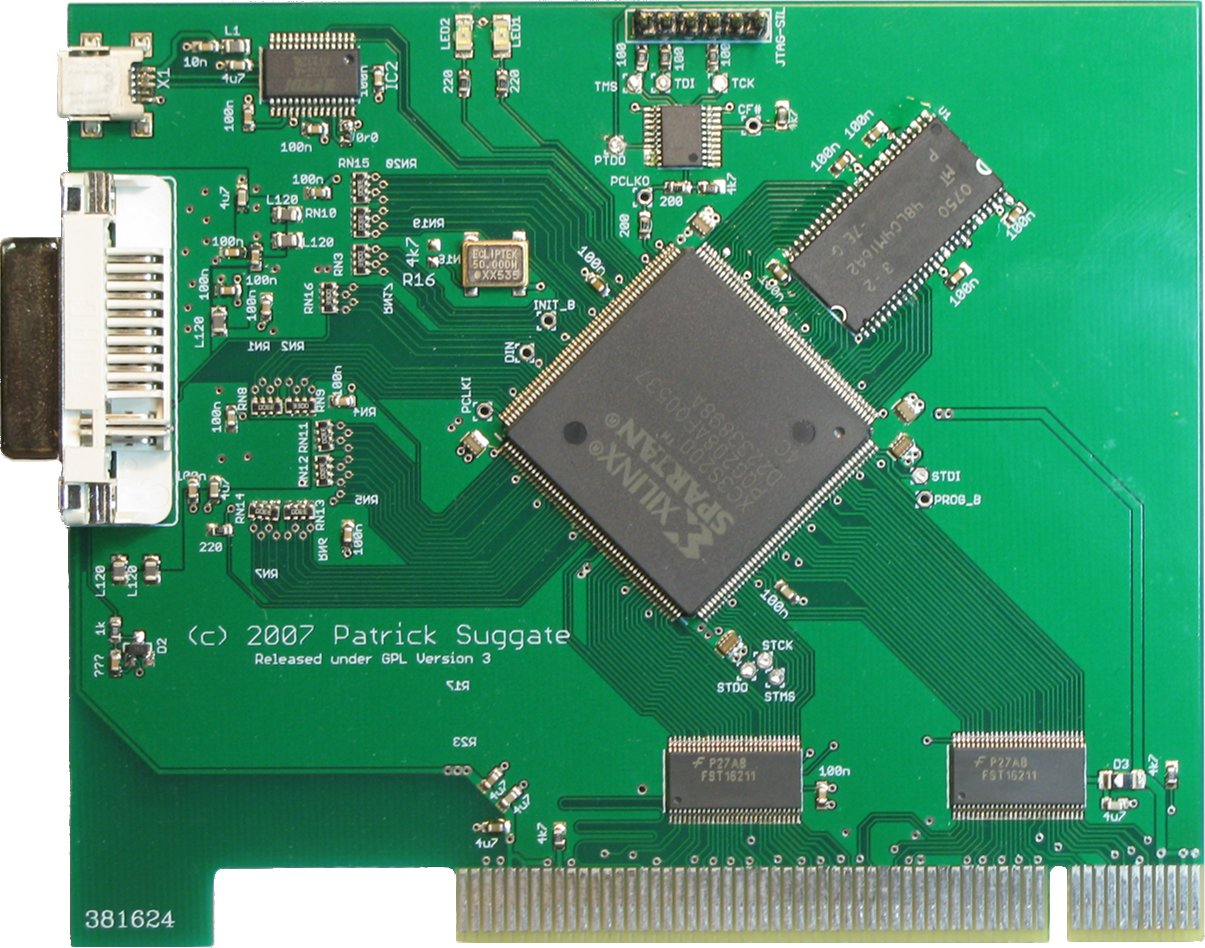
\includegraphics[width=\linewidth]{images/freega_overview.pdf}
\caption[OpenVGA Hardware Features]{OpenVGA Hardware Features.}
\label{OPENVGA_OpenVGA}
\end{center}
\end{figure}


\section{Hardware Development}
\label{OPENVGA_Hardware}

Most of the significant hardware components of OpenVGA are shown in
Figure~\ref{OPENVGA_OpenVGA}. Components not shown in this image are the VGA
video \gls{dac} and
the \gls{dvi} \gls{tmds} encoder, as these components are soldered to the reverse side of the
PCB (see Figure~\ref{HARD_Bot}). The PCB only has two copper layers to meet two
of the design goals of OpenVGA, simplicity and low-cost. A full list of all of
OpenVGA's electronic components and where to obtain the PCB artwork is found in
Appendix~\ref{HARDWARE}.

Logic cores were developed which interface to many of these hardware components.
There are logic cores implementing functionality for PCI, controlling the Video
RAM, sending and receiving via the USB UART, and encoding video data for either
DVI or VGA displays. These logic cores are introduced later in this chapter in
Section~\ref{OPENVGA_Logic_Cores}.

\begin{figure}[h]
\begin{center}
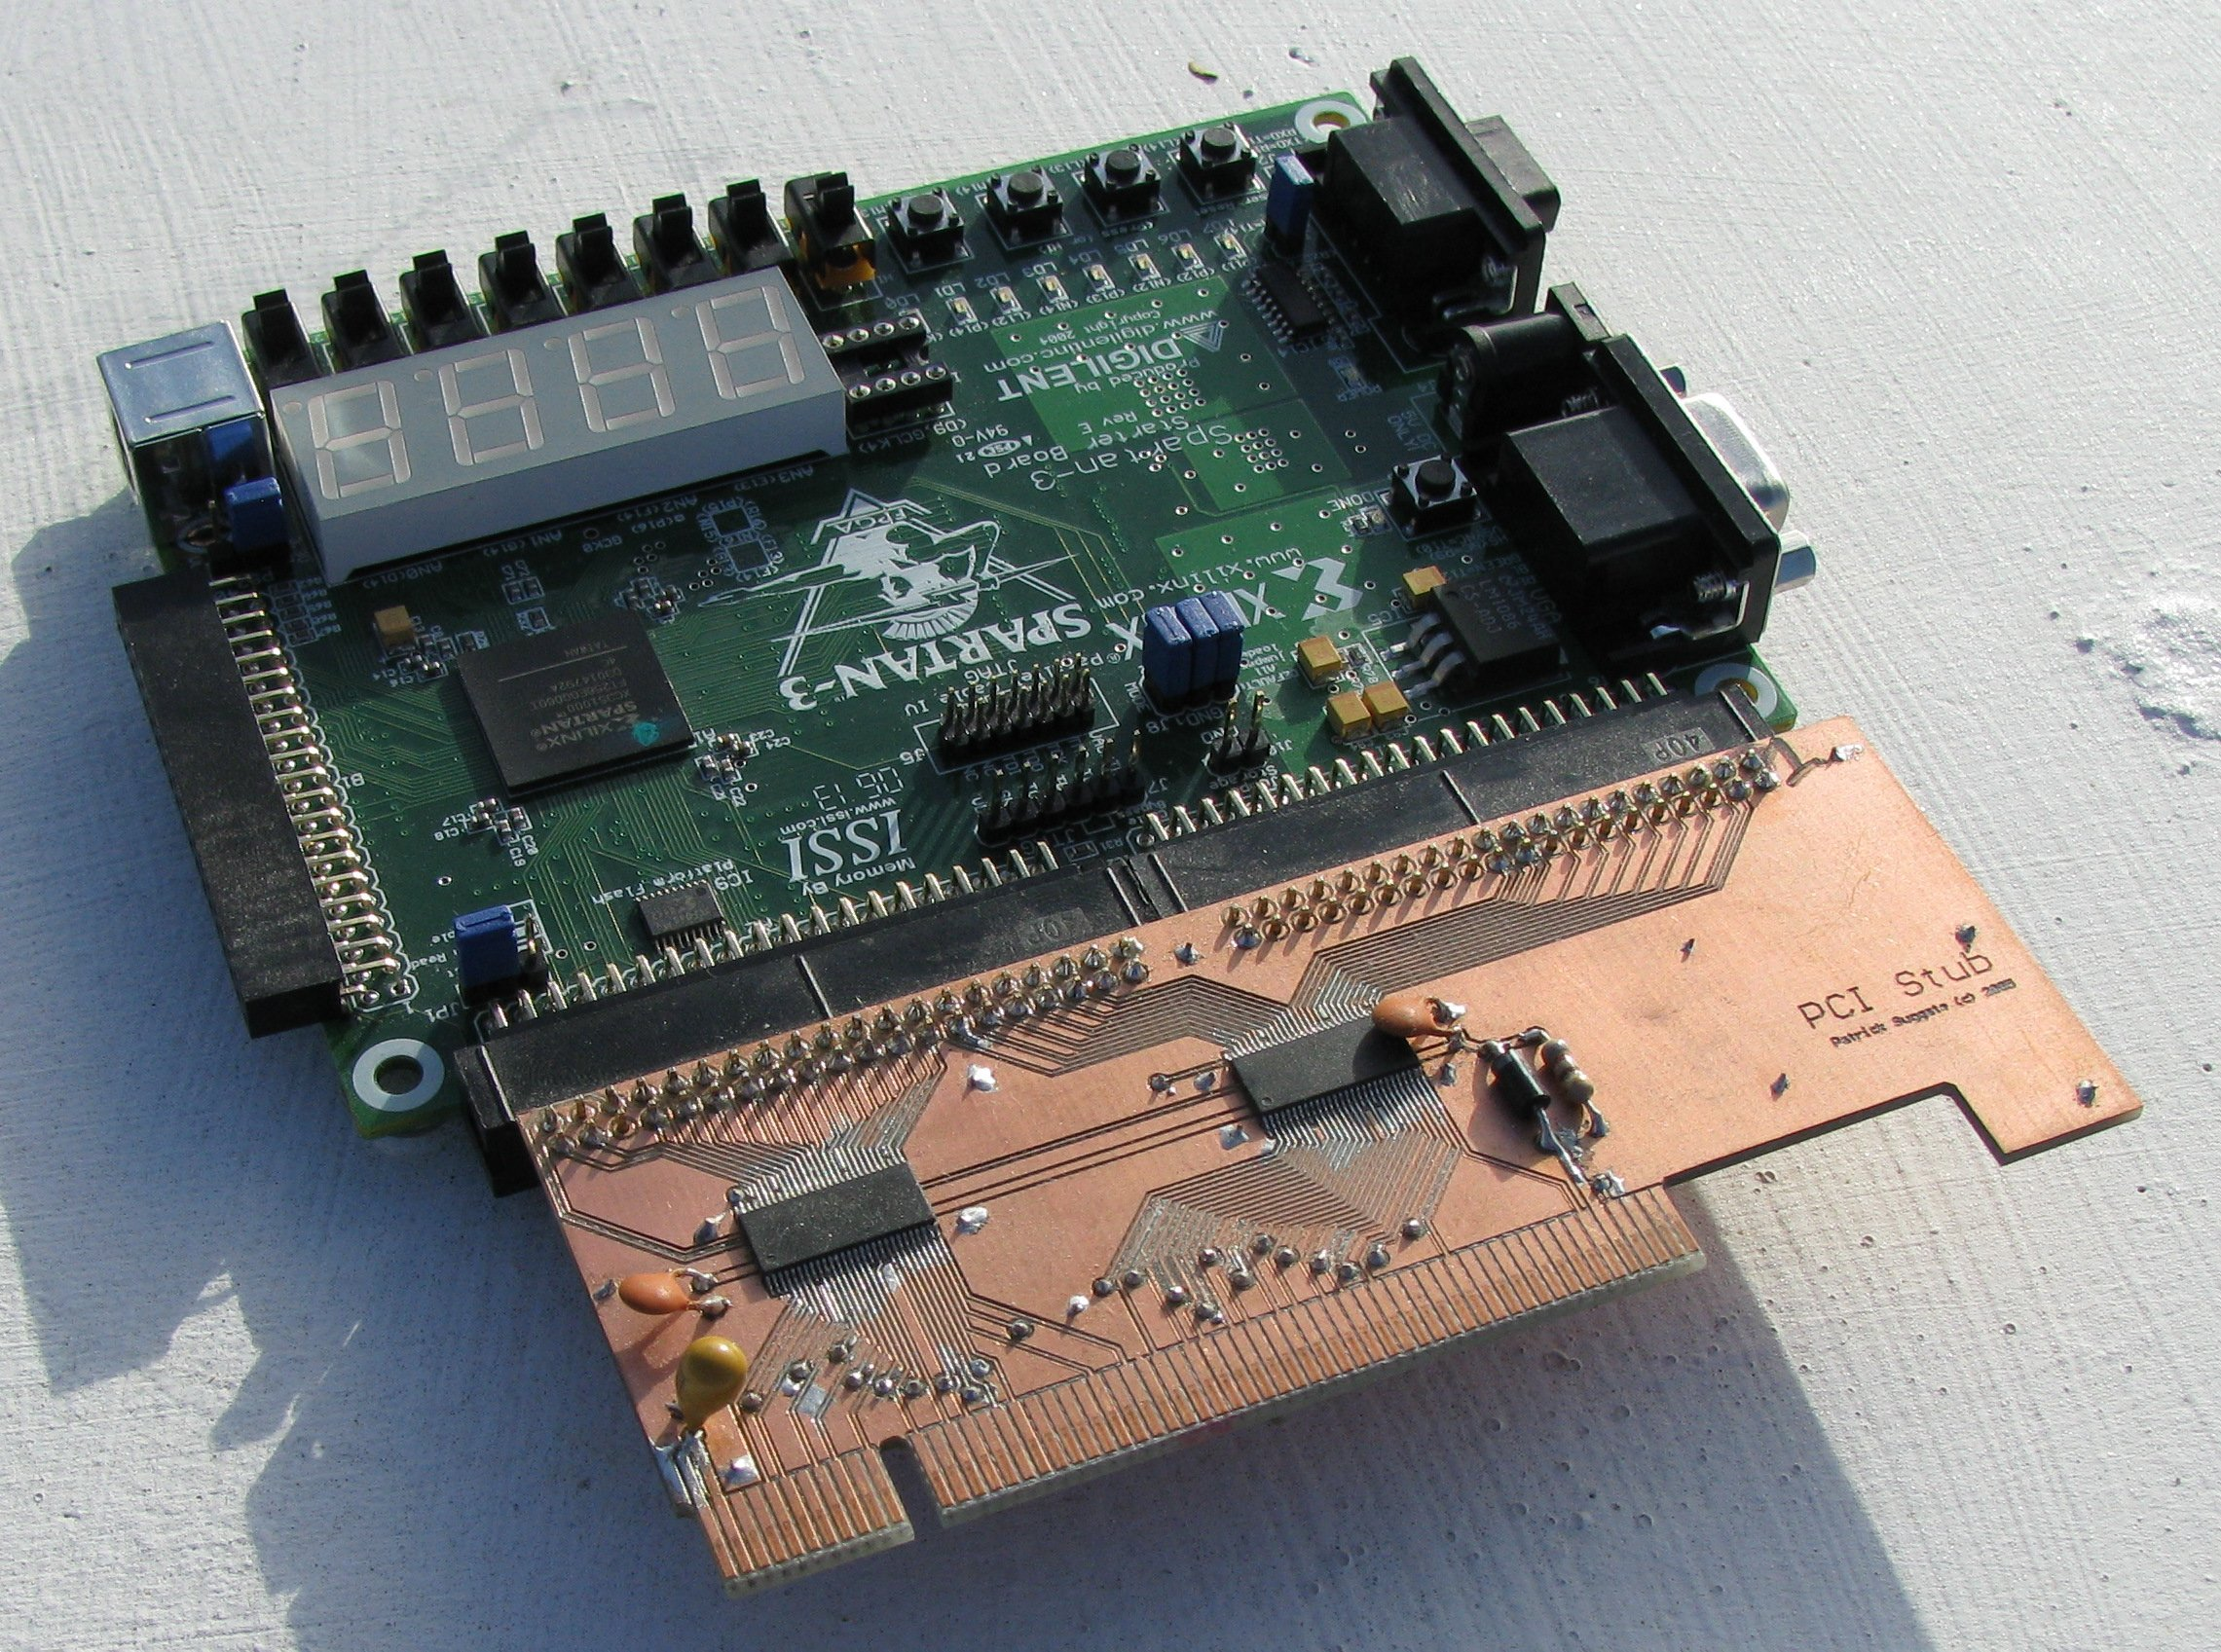
\includegraphics[width=\linewidth]{images/pci_stub.jpeg}
\caption[PCI development stub board]{PCI development stub board. The
bus-switches, which are visible in the middle of the copper coloured PCB,
translate the PCI's 5 V signals to the 3.3 V required by the Spartan-3 FPGA.}
\label{OPENVGA_PCI_Stub}
\end{center}
\end{figure}

Initial hardware development concentrated on adding PCI support to an existing
Spartan-3 development board, as shown in Figure~\ref{OPENVGA_PCI_Stub}. The PCI
logic core needed to be developed first as this allowed the host PC to run
testbenches on the logic cores which were developed later. A simple PCI stub PCB
had to be constructed (the copper-coloured board shown in the photograph). This
board contains only two ICs, just simple bus-switches to translate between the
3.3 V signalling of the Spartan-3 development board and the 5 V PCI signalling
used in many PCs.

The stub board was then connected to a commercial Spartan-3 Starter Kit
development board (the green circuit board shown in the photograph) to develop
the PCI-to-Wishbone-bridge logic core (see Sections~\ref{OPENVGA_PCI}
and~\ref{PCI}). An additional advantage of this arrangement was that the
connectors between the stub board and the development board allowed digital
oscilloscope probes to be attached. This made debugging of the PCI logic core
easier since the electrical signals of the PCI bus could be monitored during
testing (see Figure~\ref{PCI_CFG_Cap}).

\begin{figure}[h]
\begin{center}
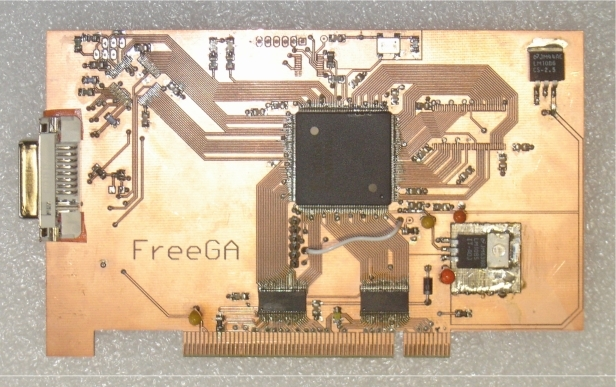
\includegraphics[width=\linewidth]{images/FreeGA_orig.jpeg}
\caption[OpenVGA PCB version 2 with DDR SDRAM]{Prototype PCB featuring DDR
SDRAM, DVI, and only eight colour VGA (via the DVI analogue outputs).}
\label{OPENVGA_Version2}
\end{center}
\end{figure}

Following this, an initial prototype board for OpenVGA was milled in-house, on a
LPKF\texttrademark~PCB milling machine, and is shown in
Figure~\ref{OPENVGA_Version2}. This board was an attempt to use Double Data
Rate (\gls{ddr}) SDRAM with
OpenVGA to provide greater memory bandwidth\footnote{The DDR SDRAM specification
requires that signal traces be terminated, since DDR SDRAM was designed to
operate at frequencies up to 200 MHz. The OpenVGA DDR version of the PCB did not
allow for these resistors since satisfactory placement would be extremely
difficult with the two-layer PCB used, since there are no ground-planes. It was
decided to attempt DDR support without termination resistors, since the
trace-lengths were very short, but DDR SDRAM could not be made to operate.}.
Though the DDR SDRAM controller was successfully simulated with the Icarus
Verilog simulator, using the Micron-provided DDR SDRAM Verilog module, the
synthesised design did not work\footnote{The DDR signals showed significant
overshoot and undershoot when monitored on an oscilloscope, and the DDR IC
produced a lot of heat.}. Due to the problems with DDR SDRAM, the final version
of the OpenVGA PCB was designed to use standard, single data-rate SDRAM (labelled
as ``Video RAM'' in Figure~\ref{OPENVGA_OpenVGA}).


\section{Important Design Elements within the FPGA}
\label{OPENVGA_Logic_Cores}
Implemented within OpenVGA's Spartan-3 FPGA are many logic cores and the
necessary bus and clocking logic. Figure~\ref{OPENVGA_Arch} shows the significant
features of the digital-logic design, and the FPGA's connectivity with the other
on-board components of OpenVGA. All logic was described using the Verilog HDL,
simulated using Icarus Verilog, and synthesised using tools which Xilinx freely
provides for use with their FPGAs.

The design contains a processor core for data processing, initialisation, and
mode-managing tasks. OpenVGA can be configured to be use either one of the two
processors that were developed for this project, TTA16 or RISC16. Additional
cores are a small data cache since memory latency is high, a SDRAM controller, a
PCI-to-Wishbone bridge, logic to read the \gls{sprom} (Serial Programmable \gls{rom}),
and numerous other support modules.

\begin{figure}[h!]
\begin{center}
\includegraphics[width=\linewidth]{images/freega_arch.pdf}
\caption[OpenVGA Architecture Block Diagram]{OpenVGA Architecture Block Diagram.}
\label{OPENVGA_Arch}
\end{center}
\end{figure}


\subsection{Logic Core Interconnection}
The Wishbone interconnect standard\footnote{Wishbone is called an
``interconnect'', instead of a ``bus'', standard as it allows for numerous
circuit topologies: buses, crossbar switches, point-to-point, and many others.}
was used as the standard interface for communication between logic cores. This
standard was designed for System-on-a-Chip (\gls{soc}) applications, is very flexible, is commonly
used with other open-source hardware projects, and requires very little logic to
implement. Appendix~\ref{APP_Wishbone} gives a brief introduction to Wishbone,
covering the core signals and providing a simple example implementation.


\subsection{FPGA-Optimised Processor Cores}
The OpenVGA initialisation, state-management, and data-processing tasks were to
be performed using a processor logic core. Existing processor logic cores were
considered but, due to performance, capability, and size requirements, two new
processors were developed for OpenVGA instead. OpenVGA requires a processor that
is be able to address at least 8 MB of memory, so this ruled out existing 8-bit
processors. The evaluated 32-bit processors were too large, so a fast 16-bit
processor was needed, but nothing suitable was found.

The first processor developed was a novel TTA processor. Significant research has
been done with this class of architecture~\cite{corporaal1993maa,
jaaskelainen2007cta}, but there are very few commercial processors of this type.
The second is a more traditional Reduced Instruction Set
Computer
(\gls{risc}) architecture processor design. It was developed to compare with TTA16, the
first OpenVGA processor. Optimised for the same tasks, both processors used the
similar functional units. This provides a good platform for the comparison of
these two architectures.


\subsubsection{TTA16}
TTA16 is a 16-bit, Wishbone-compatible, TTA processor that can operate at up to
190 MHz, and has a very small footprint\footnote{These results are for synthesis
on a Spartan-3 FPGA, and depend on the build configuration and synthesiser
optimisation settings.}. It has a fixed, 32-bit instruction word and can perform
four data transports every clock cycle. This processor is covered in detail in
Section~\ref{TTA16}, and Appendix~\ref{TTA_Programming} is a programming guide
for TTA16.


\subsubsection{RISC16}
Due to the difficulty of writing assembly code for TTA16, RISC16 was developed
and is of a more traditional design. While not as fast as TTA16, operating at up
to 140 MHz, instruction width is only 16-bits so code density is better. The
external interface is Wishbone-compatible too, and is therefore identical to
TTA16, so that this logic core can be a drop-in replacement. More detail of
RISC16 is within Section~\ref{RISC16}, and Appendix~\ref{RISCPROG} is a simple
programming guide.


\subsection{Processor Data Cache}
A low-latency, Wishbone-compatible, data cache was needed for adequate processor
memory-access performance. The 8 MB of on board memory is shared amongst multiple
logic cores, and the latency is several Wishbone cycles, so any processor access
would lead to stalls of many cycles. Both interfaces to this cache are Wishbone,
and the number of width memory-address bus is parameterisable.

Other cache features are a fast-hit path with a latency of zero cycles, a slower
hit path of one cycle of latency, operating frequency of 150 MHz, two-way
set-associativity, a line-size of 64 bytes, and a capacity of 2 kB. A full
explanation of the cache's features and design decisions is within
Section~\ref{MEM_Cache}).


\subsection{Clock Domains and Domain Crossing}
OpenVGA has multiple external interfaces and several different and asynchronous
clocks. OpenVGA has three clock domains, these are the 50~MHz Wishbone bus
domain, the 33~MHz PCI Local Bus domain, and the dot-clock domain. While the PCI
bus typically operates at a frequency of 33 MHz, though this is not guaranteed,
and this clock signal is driven by the system host. The dot-clock of display
circuitry depends upon the video mode, as higher resolutions require more pixels
be drawn, therefore requiring a higher pixel rate. Currently the dot-clock can be
selected as either 25 MHz or 40 MHz (see Section~\ref{VIDEO_Modes}).

As well as asynchronous clock domains, some components of OpenVGA run at integer
multiples of the Wishbone domain's 50 MHz clock rate, the SDRAM and RISC16
operate at 100 MHz, and TTA16 operates at 150 MHz. These clocks are synchronous
with the Wishbone clock and present fewer problems. A further explanation and
solutions are covered in Section~\ref{CLOCK_Sync}.

When logic cores have different clocks, data must be synchronised when passing
from one core to the other. When the clocks are asynchronous this becomes even
more difficult due to metastability issues. A D-type
Flip-Flop (\gls{dff}) can enter a
metastable state\footnote{This metastable state means that the output of the DFF
is essentially random, but it oscillates for a significant time before it settles
back into a stable state~\cite{Async_FIFO2}.} when setup and/or hold times are
violated. Section~\ref{CLOCK} presents the OpenVGA clock architecture and
domains, examines the problems with domain crossing, and presents the solutions
used to solve these. Asynchronous First-In, First-Out
queues (\gls{fifo}s) allow
signals that are multiple bits wide to be synchronised across clock domains and
are presented in Section~\ref{CLOCK_Async_FIFO}.


\subsection{Memory Controller}
\label{OPENVGA_Mem_Ctrl}
A high performance, small logic foot-print, Wishbone-compatible memory controller
was needed for OpenVGA. Tasks the controller has to perform include refreshing
the DRAM, support burst reads and writes, and atomic reads and writes. To
minimise the size of the controller it has to operate within the Wishbone clock
domain so that asynchronous FIFOs are not needed.

The SDRAM data transfers occur at 100 MHz while the controller's state machine
operates at 50 MHz, the Wishbone memory bus frequency. This was achieved by using
the DDR input and output primitives within the Spartan-3 I/O
Blocks (\gls{iob}s).
Section~\ref{MEM_SDRAM} provides more detail on the controller, including the
design of the state machine and data path implementations.


\subsection{PCI-to-Wishbone Bridge}
\label{OPENVGA_PCI}
A small PCI-to-Wishbone-bridge logic core was developed so that the system host
can communicate with OpenVGA. This bridge supports the ``Plug and Play'' standard
and Memory-mapped I/O (\gls{mmio}), which maps the OpenVGA SDRAM into the host PC's memory
address space. Only the PCI Local Bus features that were needed for OpenVGA are
implemented and resulted in a design about one-tenth the size of another
available open-source PCI bridge\footnote{There is a very capable, FPGA-tested,
PCI bridge available over the Internet from OpenCores site.}. The design of the
bridge, descriptions of its state-machines, and domain crossing issues are
explained Section~\ref{PCI}, and more details of the clock domain issues are
covered in Section~\ref{CLOCK}.

So that the host OS can access OpenVGA, a simple Linux kernel module was written.
Linux kernel modules are written using the C programming language\footnote{A
comprehensive guide to developing Linux kernel modules is available
from~\cite{salzman:lkm}.} and OpenVGA is accessed from the GNU/Linux OS by
opening the device file which represents the MMIO of OpenVGA. Using read, write,
and seek operations, any location within the OpenVGA SDRAM can be read and
written.


\subsection{VGA/LCD Display Controller}
This logic core prefetches image data from the memory controller, using the
system's memory Wishbone bus, and generates the timing signals and bit-streams
necessary for driving VGA and LCD displays (see Section~\ref{VIDEO}). The
Wishbone bus can be in a different clock domain to the dot-clock since an
asynchronous FIFO is used for the prefetch logic. This has a 2 kB prefetch
capability and is discussed in more detail in Section~\ref{VID_Prefetch}.

Within the display controller is a CRT controller which has registers that can be
accessed using a Wishbone interface. This allows the timing parameters to be set
allowing the display mode to be changed (see Section~\ref{VID_CRTC}).


\subsection{Additional Logic Cores}
Other smaller logic cores were developed for OpenVGA. Detailed explanations of
these can be found within Chapters~\ref{MEM} (Memory) and~\ref{IO_Chapter}
(I/O), and a summary of these is:

\begin{itemize}
  \item USB UART: A Wishbone-compatible interface to a 9600 baud UART which
  communicates with the on-board FTDI FT232R USB UART IC. More detail can be
  found in Section~\ref{USB_Sport}.
  \item LED driver: There are two Wishbone-mapped LEDs that can be set and
  cleared using this module, covered further in Section~\ref{LED_Driver}.
  \item DMA controller: A simple Direct Memory Access controller is used to
  improve the memory write performance of OpenVGA's processor. This logic core
  is detailed in~\ref{MEM_DMA} and a programming guide for it is in
  Appendix~\ref{TTAPROG_DMA}.
  \item Serial PROM reader: Spartan-3 FPGAs require configuration upon
  power-on. The on-board serial PROM contains this configuration data but also
  has enough capacity to store some extra data. This module can read this data
  from the SPROM when requested via its Wishbone interface.
  Section~\ref{Serial_PROM} presents more information on this module.
\end{itemize}
